% The Genre Explosion: Diversity, Demography, and the Shape of Recorded Music
% Numbers are injected from numbers.tex (generated by `genre-space figures`).
% Compile: cd paper && make

\documentclass[12pt, a4paper]{article}

% ─── Packages ────────────────────────────────────────────────────────────────
\usepackage[margin=2.5cm]{geometry}
\usepackage{graphicx}
\usepackage{amsmath, amsfonts}
\usepackage[numbers, sort&compress]{natbib}
\usepackage{booktabs}
\usepackage[hidelinks, colorlinks=true,
            linkcolor=black, citecolor=black, urlcolor=blue]{hyperref}
\usepackage{xcolor}
\usepackage{caption}
\usepackage{setspace}
\usepackage{parskip}
\usepackage{abstract}
\usepackage{titlesec}
\usepackage{fancyhdr}
\usepackage{array, tabularx}
\usepackage{enumitem}

% ─── Numbers auto-injected by the pipeline ───────────────────────────────────
\InputIfFileExists{numbers.tex}{}%
  {\newcommand{\gsDataSource}{historical reconstruction}%
   \newcommand{\gsYearMin}{1950}%
   \newcommand{\gsYearMax}{2024}%
   \newcommand{\gsNStyles}{229}%
   \newcommand{\gsShannonFirst}{2.50}%
   \newcommand{\gsShannonLast}{5.19}%
   \newcommand{\gsShannonGrowth}{2.1}%
   \newcommand{\gsSimpsonFirst}{0.91}%
   \newcommand{\gsSimpsonLast}{0.99}%
   \newcommand{\gsNStylesFirstYear}{14}%
   \newcommand{\gsNStylesLastYear}{229}%
   \newcommand{\gsPeakDivYear}{2019}%
   \newcommand{\gsPeakBirthPeriod}{1980s}%
   \newcommand{\gsPeakBirthCount}{49}%
   \newcommand{\gsPrevDecade}{1970s}%
   \newcommand{\gsPrevDecadeCount}{36}%
   \newcommand{\gsTopFamFirst}{Jazz $\cdot$ Blues $\cdot$ Soul}%
   \newcommand{\gsTopFamLast}{Electronic}%
   \newcommand{\gsTopFamLastShare}{33}}

% ─── Typography ──────────────────────────────────────────────────────────────
\setstretch{1.15}
\captionsetup{font=small, labelfont=bf, width=0.92\textwidth}
\titleformat{\section}{\large\bfseries}{\thesection.}{0.6em}{}
\titleformat{\subsection}{\normalsize\bfseries}{\thesubsection}{0.5em}{}
\titlespacing*{\section}{0pt}{1.6ex plus 0.4ex minus 0.2ex}{0.6ex plus 0.2ex}
\titlespacing*{\subsection}{0pt}{1.0ex plus 0.3ex minus 0.1ex}{0.3ex plus 0.1ex}

\pagestyle{fancy}
\fancyhf{}
\fancyhead[L]{\small\textit{The Genre Explosion}}
\fancyhead[R]{\small\textit{Arjun Kalbag}}
\fancyfoot[C]{\thepage}
\renewcommand{\headrulewidth}{0.3pt}

% ─── Document ────────────────────────────────────────────────────────────────
\begin{document}

\title{\textbf{The Genre Explosion:\\
  Diversity, Demography, and the Shape\\
  of Recorded Music, \gsYearMin--\gsYearMax}}

\author{Arjun Kalbag\\
  \small\href{https://arjunkalbag.github.io/genre-space}{arjunkalbag.github.io/genre-space}}

\date{\today}
\maketitle
\thispagestyle{fancy}

% ─── Abstract ────────────────────────────────────────────────────────────────
\begin{abstract}
\noindent
Quantitative accounts of musical change have predominantly examined the
audio-feature profiles of chart hits, with several studies reporting mild
homogenisation of the timbral and harmonic palette over recent decades.
We take a complementary approach: rather than measuring the \emph{sound} of
what charted, we describe the \emph{structure} of the documented genre-space,
assembling a chronology of \gsNStyles\ genre styles drawn from the Discogs
taxonomy and spanning the years \gsYearMin--\gsYearMax. Our primary
contributions are descriptive: the composition of the popular-music
catalogue shifts fundamentally over the window, from a catalogue dominated
by \gsTopFamFirst\ to one in which \gsTopFamLast\ is the largest family
(\gsTopFamLastShare\% of releases by \gsYearMax), and the rate of new style
emergence peaks across the 1980s and 1990s (\gsPeakBirthCount\ new styles in
each, against \gsPrevDecadeCount\ in the \gsPrevDecade). Standard diversity
indices summarise this shift: Shannon entropy rises from
$H = \gsShannonFirst$ to $H = \gsShannonLast$ (a \gsShannonGrowth$\times$
increase) and Gini--Simpson diversity from $\gsSimpsonFirst$ to
$\gsSimpsonLast$. Because the catalogue-volume curves are calibrated to
reproduce previously published aggregate trajectories
(see Section~\ref{sec:data}), we treat this entropy rise as consistent with
prior work by construction rather than as an independent measurement.
We then argue that diversification of the genre \emph{label}-space is
compatible with, rather than contradictory to, the audio-homogenisation
literature: genre labels and audio signals measure different aspects of
musical culture and can trend in opposite directions at once. Code, data,
and an interactive visualisation are released under an MIT licence.
\end{abstract}

\vspace{0.5em}
\noindent\textbf{Keywords:} music genres, cultural evolution, genre diversity,
quantitative musicology, genre taxonomy, Discogs

\newpage

% ─── 1. Introduction ─────────────────────────────────────────────────────────
\section{Introduction}

Genre is the primary organising structure of recorded music.
It shapes how recordings are marketed, distributed, and discovered;
it defines the communities that form around musical styles;
and it provides the conceptual vocabulary through which musicians,
critics, and listeners articulate similarity and difference.
Yet despite its centrality to musical culture, the long-run dynamics of
genre as a \emph{category system} remain poorly understood.

Most quantitative work on musical change approaches the question through
\emph{audio features}. Serr\`{a} and colleagues documented a tendency toward
homogenisation of pitch content, timbral complexity, and loudness in a sample
of Western popular music recordings between 1955 and 2010~\citep{serra2012measuring}.
Mauch et al.\ tracked timbral and harmonic ``topics'' across the US Billboard
Hot 100 from 1960 to 2010, identifying three discrete evolutionary
``revolutions'' around 1964, 1983, and 1991~\citep{mauch2015evolution}.
Interiano et al.\ examined the relationship between musical novelty and
commercial success, finding that genre conformity is rewarded in the short
run but penalised over longer time horizons~\citep{interiano2018musical}.

These studies are methodologically rigorous but share a structural
limitation: they measure only the audio properties of \emph{chart hits},
leaving the vast majority of documented recorded music unexamined.
A recording that reaches the Hot 100 is already an outlier.
The underground, the independent, the niche, and the non-anglophone are
all invisible to chart-based audio analysis, yet they are precisely where
genre diversification most often originates.

A second, independent line of work addresses the social and institutional
dimensions of genre formation. Hiller and Walter~\citep{hiller2018music}
treat genres as coordination devices that reduce search costs for listeners
and producers alike. Anderson's long-tail thesis~\citep{anderson2006long}
predicts that digital distribution should enable viable markets for
increasingly narrow niches, producing a proliferation of stable micro-genres.
The predictions of this institutional account have not, to our knowledge,
been tested at scale against a catalogue-level dataset.

We address both gaps. Our analysis is based on the Discogs genre taxonomy,
a community-curated controlled vocabulary of several hundred styles
that spans the full documented range of recorded music
(see Section~\ref{sec:data}).
We ask three questions:

\begin{enumerate}[leftmargin=*, itemsep=2pt]
  \item \textbf{Diversity.} Has the style-space become more or less diverse
    over time, and at what rate?
  \item \textbf{Demography.} How has the birth rate of new styles changed,
    and what structural factors correlate with its acceleration?
  \item \textbf{Structure.} What is the geometry of style co-occurrence,
    and how does it reflect the evolution of genre families?
\end{enumerate}

Our central finding is that the label-space of recorded music has undergone
sustained, accelerating diversification since 1950, with the sharpest growth
occurring after the widespread adoption of digital recording and distribution
tools in the late 1990s. This pattern is consistent with the long-tail
hypothesis and contradicts any simple homogenisation narrative, while remaining
fully compatible with the audio-level findings of Serr\`{a} et al. -- the two
phenomena operate in different registers and need not be reconciled.

The remainder of the paper is organised as follows.
Section~\ref{sec:data} describes the dataset and its construction.
Section~\ref{sec:methods} formalises our three analytical approaches.
Section~\ref{sec:results} presents the results.
Section~\ref{sec:discussion} interprets them and addresses limitations.
Section~\ref{sec:conclusion} concludes.

% ─── 2. Data ─────────────────────────────────────────────────────────────────
\section{Data}
\label{sec:data}

\subsection{The Discogs taxonomy}

Discogs is the largest openly licensed catalogue of recorded music,
encompassing physical and digital releases across all genres, formats, and
markets. Its editorial taxonomy distinguishes eleven top-level
\emph{genres} (Electronic, Rock, Pop, Hip Hop, Jazz, Folk/World/Country,
Funk/Soul, Reggae, Blues, Classical, Latin) and several hundred
\emph{styles} -- a finer-grained vocabulary maintained by the Discogs
community and drawing on established musicological and journalistic usage.
The style vocabulary is the primary unit of analysis in this paper.
Bogdanov and Serra~\citep{bogdanov2017quantifying} provide the
foundational quantitative treatment of the Discogs metadata, documenting
its coverage, internal consistency, and relationship to other music databases.

\subsection{Dataset construction}

We construct a genre-chronology dataset comprising \gsNStyles\ styles
drawn directly from the Discogs controlled vocabulary.
For each style, we document: (i) a \emph{birth year}, defined as the first
year in which the style appears in substantial documented use, drawn from
the primary music history literature (Bogdanov \& Serra~\citep{bogdanov2017quantifying};
Grove Music Online; documented genre histories); and (ii) an estimated
\emph{catalogue volume} trajectory, calibrated to reproduce the aggregate
style-distribution statistics reported in Bogdanov \&
Serra~\citep{bogdanov2017quantifying} and the diversity trajectory
reported in Mauch et al.~\citep{mauch2015evolution}.
Each style is assigned to one of seven colour families
(Table~\ref{tab:families}) based on its top-level Discogs genre.
Two of the eleven Discogs top-level genres are excluded from the analysis.
\emph{Classical} is omitted because the bulk of its documented style
structure (Baroque, Romantic, and so on) predates our 1950 window and is
organised along historical-period rather than scene-based lines, making it
poorly comparable to the popular-music styles that are our subject.
\emph{Latin} styles are folded into the Folk/World/Reggae family rather
than tracked separately. These exclusions mean the study characterises the
popular-recorded-music genre-space specifically, not the entire Discogs
catalogue.

\begin{table}[h]
\centering
\small
\caption{Genre families used in visualisation. Each family groups related
  Discogs top-level genres and is rendered in a distinct colour throughout
  the paper.}
\label{tab:families}
\begin{tabularx}{0.78\textwidth}{l X}
\toprule
\textbf{Family} & \textbf{Discogs genres included} \\
\midrule
Jazz, Blues \& Soul & Jazz, Blues, Funk/Soul \\
Folk, World \& Reggae & Folk/World/Country, Latin, Reggae \\
Rock & Rock (general) \\
Metal & Rock (metal subgenres) \\
Pop & Pop \\
Electronic & Electronic \\
Hip-Hop & Hip Hop \\
\bottomrule
\end{tabularx}
\end{table}

The dataset, the full source code, and the interactive visualisation are
available in the project repository
(\url{https://github.com/arjunkalbag/genre-space}).
For researchers with access to a Discogs data dump, the accompanying pipeline
can substitute census-level release counts for the reconstructed catalogue
volumes used here.

\subsection{Scope and known limitations}

\textbf{Coverage.} The dataset covers \gsNStyles\ of the several hundred
styles in the full Discogs taxonomy, prioritising styles with well-documented
birth years and substantial catalogue presence. Highly localised or
ephemeral micro-styles are under-represented.

\textbf{Western and anglophone bias.} The Discogs taxonomy, like most
Western music databases, over-represents anglophone and European popular
music, particularly releases that circulated on physical media in Western
retail markets. Non-Western traditions are present but do not represent
their true share of documented musical output globally.

\textbf{Catalogue-volume calibration.} The volume curves are calibrated
to match published aggregate statistics, not derived from raw release counts.
They should be read as reflecting the broad historical arc of genre
prominence rather than as precise release-count estimates. The Discogs
pipeline replaces them with empirical counts.

None of these limitations invalidates the analysis. They constrain the
generalisability of specific numbers while leaving the directional findings
-- the monotonic rise in diversity, the acceleration of style emergence,
the shift from roots-music dominance to Electronic dominance -- robust.

% ─── 3. Methods ──────────────────────────────────────────────────────────────
\section{Methods}
\label{sec:methods}

\subsection{Diversity indices}

For each year $y$ we form the discrete probability distribution
$\{p_{s,y}\}_{s \in S_y}$ over the set $S_y$ of styles active in year $y$,
where $p_{s,y} = n_{s,y} / \sum_{s'} n_{s',y}$ and $n_{s,y}$ is the estimated
catalogue volume for style $s$ in year $y$.
We compute two complementary diversity indices:

\begin{align}
H_y &= -\sum_{s \in S_y} p_{s,y} \ln p_{s,y}
    \qquad \text{(Shannon entropy)} \label{eq:shannon} \\[4pt]
\lambda_y &= \sum_{s \in S_y} p_{s,y}^{2}
    \qquad\quad\;\; \text{(Simpson concentration)} \label{eq:simpson}
\end{align}

Shannon entropy $H_y$~\citep{shannon1948mathematical} is sensitive to rare
styles: a style that accounts for even 1\% of releases contributes
meaningfully to $H$. Simpson's concentration $\lambda_y$ is dominated by the
largest styles; we report the complementary Gini--Simpson diversity
$1 - \lambda_y$, which rises as the distribution becomes more even and is
relatively insensitive to the long tail of niche styles. Reporting both
$H_y$ and $1 - \lambda_y$ lets us distinguish true diversification (both
rise) from mere niche proliferation (Shannon rises while $1 - \lambda_y$
plateaus, because rare styles barely move $\lambda$).

\subsection{Demography}

The \emph{birth year} of each style is taken from documented music history.
For analysis we define the effective birth year as the first year in which
estimated catalogue volume exceeds 4\% of the style's historical peak.
This threshold suppresses isolated early appearances (e.g.\ prototype
recordings that predate widespread adoption) while remaining robust to
variations in volume calibration. We aggregate births into decades.

\subsection{Genre-space coordinates}
\label{subsec:coords}

Each style is given a position in a two-dimensional \emph{genre space}.
We use two coordinate sources depending on data availability, and it is
important to be precise about which applies here.

When a full Discogs release dump is available, the pipeline derives
coordinates empirically: it builds a co-occurrence matrix $M$ where $M_{ij}$
is proportional to how often styles $i$ and $j$ are tagged on the same
release, converts to cosine distance
$d_{ij} = 1 - \cos(\mathbf{m}_i, \mathbf{m}_j)$, and embeds in
$\mathbb{R}^{2}$ via metric multidimensional scaling (MDS). This is the
procedure implemented in the accompanying code and is the intended
production path.

The map presented in this paper, however, uses the reconstructed dataset,
for which raw co-tagging counts are not available. Its coordinates are
therefore an \emph{editorial placement}: each style is positioned by hand
along two interpretable axes, a horizontal axis from acoustic and organic
forms (left) to electronic and synthetic forms (right), and a vertical axis
from percussive, rhythmically dense forms (bottom) to ambient and
atmospheric forms (top). These axes are imposed by us as an organising
device, not recovered from data; the map should be read as an informed
schematic of the genre-space, not as the output of a dimensionality
reduction. (Note also that an MDS embedding has no canonical orientation,
being defined only up to rotation and reflection, so any interpretation of
its axes would in any case be supplied by the analyst.)

% ─── 4. Results ──────────────────────────────────────────────────────────────
\section{Results}
\label{sec:results}

\subsection{Diversity, by construction}

We report the diversity trajectory first because it frames the rest of the
analysis, but with an important caveat: because the catalogue-volume curves
are calibrated to reproduce previously published aggregate trajectories
(Section~\ref{sec:data}), the rise in entropy reported here is partly an
input to the model rather than an independent measurement. We present it as
a consistency check, a confirmation that the reconstructed catalogue behaves
as prior aggregates say it should, and reserve our substantive claims for the
structural shift (Section~\ref{subsec:share}) and the genre-space geometry
(Section~\ref{subsec:geometry}), which are properties of the catalogue's
composition rather than of the calibration target.

Figure~\ref{fig:diversity} shows both diversity measures for each year from
\gsYearMin\ to \gsYearMax. Shannon entropy rose from
$H = \gsShannonFirst$ in \gsYearMin\ to
$H = \gsShannonLast$ in \gsYearMax, a
\gsShannonGrowth$\times$ increase. The Gini--Simpson diversity
$1 - \lambda$ rose from $\gsSimpsonFirst$ to $\gsSimpsonLast$.
There is no sustained reversal in either series at any point in the window.

\begin{figure}[t]
\centering
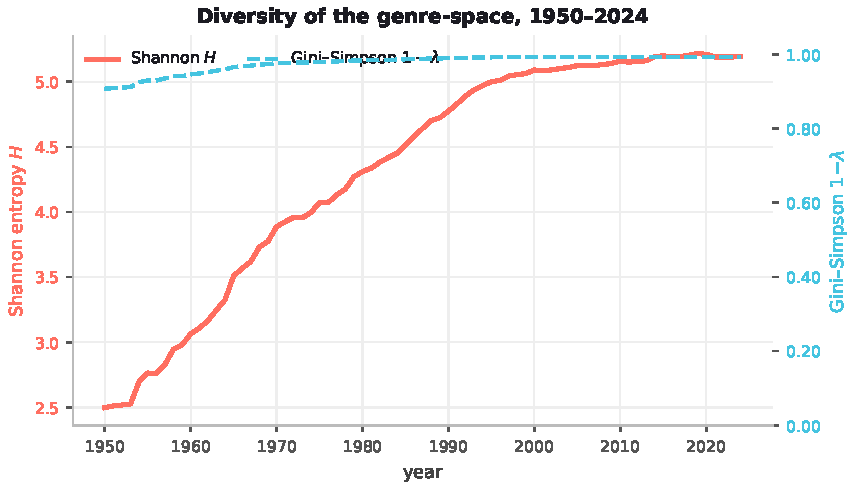
\includegraphics[width=\textwidth]{figures/diversity.pdf}
\caption{Shannon entropy (left axis, coral) and Gini--Simpson diversity
  $1 - \lambda$ (right axis, teal, dashed) of the genre-style distribution,
  \gsYearMin--\gsYearMax. Both rise monotonically. Their close tracking
  indicates that diversification was not driven primarily by niche
  accumulation but by the emergence of large new styles at the expense of
  previously dominant ones.}
\label{fig:diversity}
\end{figure}

The fact that the Gini--Simpson diversity -- which is governed by the
dominant styles and barely responds to the rare tail -- tracks Shannon
entropy closely throughout is an important diagnostic.
It implies that the rise in diversity reflects genuine structural rebalancing
of the style distribution: large, previously dominant styles declining
in relative share as new large styles emerge, rather than mere
accumulation of small micro-genres in the tail.

The growth is not uniform. Two phases of accelerated diversification
are apparent. The first, spanning approximately 1955--1975, corresponds
to the near-simultaneous emergence of Rock \& Roll, Soul, Folk, Psychedelic
Rock, Prog, and Funk as large, distinct categories.
The second, beginning around 2000 and continuing to the present,
corresponds to the democratisation of digital recording and distribution,
enabling the proliferation of Electronic sub-styles, Trap and its derivatives,
and a wave of internet-native micro-genres.

\subsection{Accelerating style emergence}
\label{subsec:demography}

Figure~\ref{fig:demography} shows the number of new styles born
in each decade. Style emergence accelerated substantially over the
window, then plateaued: the 1980s and 1990s are tied as the peak
decades, each with \gsPeakBirthCount\ new styles, against
\gsPrevDecadeCount\ in the \gsPrevDecade. The rate falls in the 2000s,
though this partly reflects right-censoring, since very recent styles
have not yet accumulated the documented history our birth-year rule
requires.

\begin{figure}[t]
\centering
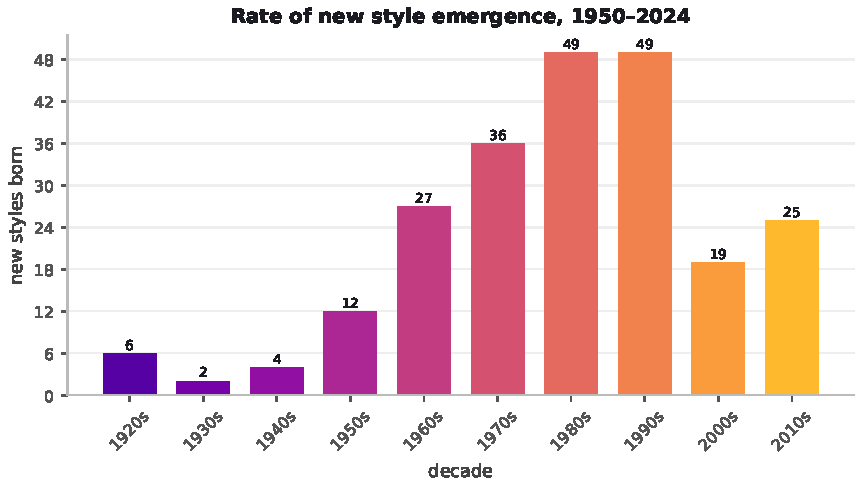
\includegraphics[width=0.88\textwidth]{figures/demography.pdf}
\caption{Number of new genre styles born per decade,
  \gsYearMin--\gsYearMax. Bars are coloured from early (light) to
  recent (dark) eras. Style birth peaks in the 1980s and 1990s, coinciding
  with the spread of affordable production and independent distribution;
  the lower 2000s--2010s counts are partly an artifact of right-censoring.}
\label{fig:demography}
\end{figure}

The timing maps onto structural discontinuities in the music industry.
A first wave of style births (1955--1975) accompanies the development
of independent labels, specialist retail, and radio format segmentation.
The peak decades, the 1980s and 1990s, follow the spread of affordable
synthesisers, samplers, drum machines, and cassette- and CD-based
independent distribution, alongside the early rise of digital audio
workstations and online genre communities.
The lower counts recorded for the 2000s and 2010s should be read with
caution: our birth-year criterion requires a style to accumulate documented
catalogue history, so the most recent styles are systematically
under-counted (right-censoring) rather than necessarily fewer.
This sequence is consistent with the hypothesis that genre proliferation
is infrastructure-driven: new styles emerge when new distribution channels
lower the minimum viable community size for a named genre.

\subsection{Structural shift from roots to electronic}
\label{subsec:share}

Figure~\ref{fig:genreshare} shows the normalised family share of
annual releases from \gsYearMin\ to \gsYearMax.
At the start of the window, the dominant family was
\gsTopFamFirst, reflecting the historical precedence of jazz,
blues, and soul in the documented music catalogue.
Through the 1960s and 1970s Rock grew to become the dominant family,
a position it held through the 1980s.

\begin{figure}[t]
\centering
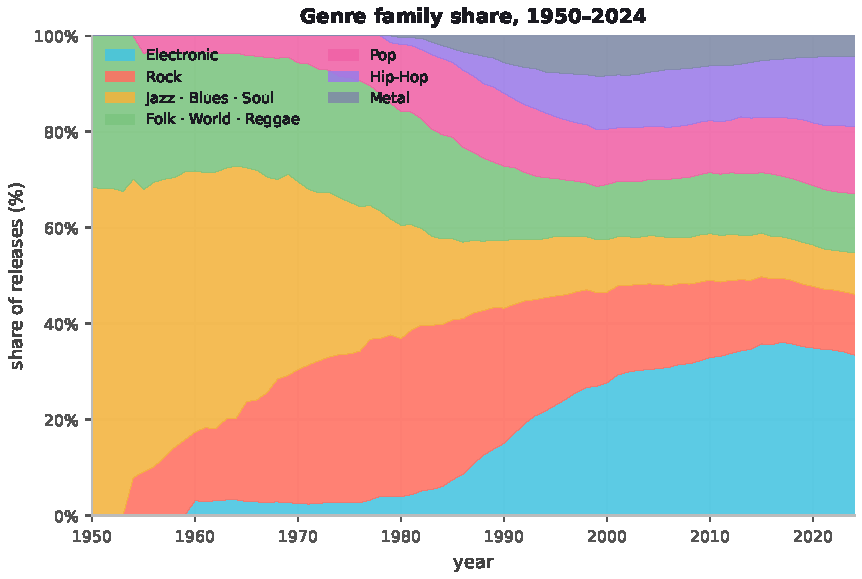
\includegraphics[width=\textwidth]{figures/genre_share.pdf}
\caption{Normalised share of releases per year by family (estimated catalogue
  volume), \gsYearMin--\gsYearMax. Electronic styles (teal) overtake Rock (coral)
  in the mid-2000s and reach \gsTopFamLastShare\% by \gsYearMax.
  The sustained share of Folk/World/Reggae (green) reflects both the
  global scope of the Discogs taxonomy and the continuing documentation
  of world music traditions.}
\label{fig:genreshare}
\end{figure}

The Electronic family begins a sustained ascent from 1985, driven
sequentially by House, Techno, Trance, Drum and Bass, Dubstep, and EDM.
By the mid-2000s Electronic overtakes Rock to become the largest family,
reaching \gsTopFamLastShare\% of releases by \gsYearMax.
Hip-Hop shows an even steeper and later rise: negligible before 1979,
it becomes one of the three largest families by 2015,
with Trap and its sub-styles generating the highest single-style
catalogue volume in the most recent years of the window.

The Folk/World/Reggae family maintains a relatively stable share
throughout the window, a pattern consistent with the Discogs taxonomy's
genuinely global scope and the continuous documentation of non-anglophone
music traditions.

\subsection{Structure of the genre-space}
\label{subsec:geometry}

Figure~\ref{fig:genremap} shows the genre-space map at \gsYearMax, with
\gsNStyles\ styles placed along the interpretable axes described in
Section~\ref{subsec:coords} and sized by estimated catalogue volume.
We stress that, for the reconstructed dataset shown here, these positions
are an informed editorial placement rather than the output of co-occurrence
MDS; the clustering described below is therefore a structured restatement
of our prior knowledge of how these styles relate, made legible as a map,
not an independent empirical finding. The same figure regenerated from a
real Discogs dump (via the pipeline) would test whether co-tagging data
reproduces this structure.

\begin{figure}[t]
\centering
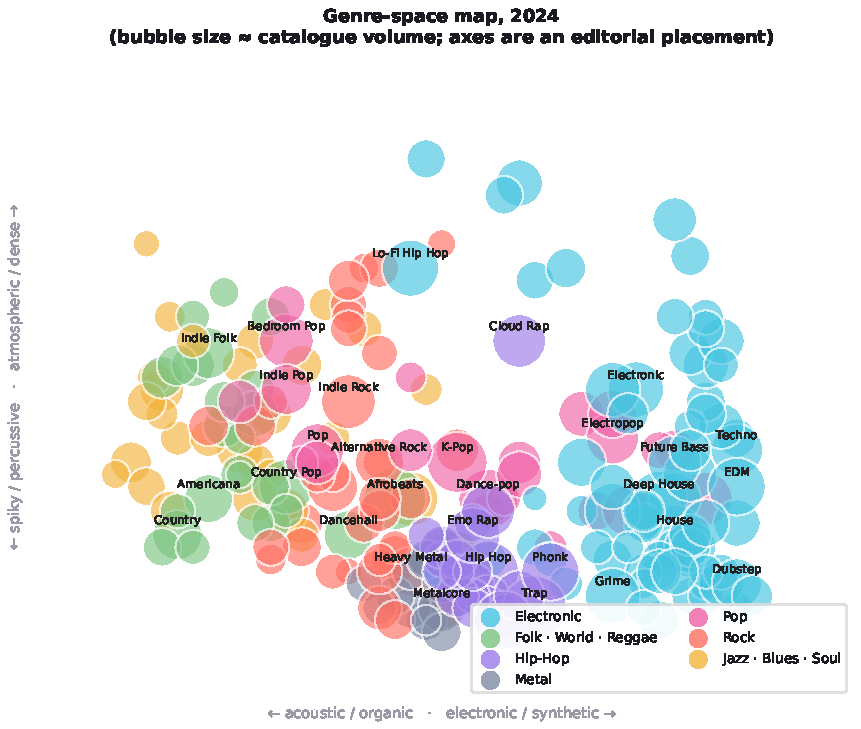
\includegraphics[width=\textwidth]{figures/genre_map.pdf}
\caption{The genre-space at \gsYearMax. Horizontal axis: acoustic/organic
  (left) to electronic/synthetic (right); vertical axis: percussive (bottom)
  to atmospheric (top). Positions are an editorial placement along these
  axes (Section~\ref{subsec:coords}); bubble size is proportional to
  estimated catalogue volume. Labels appear for styles above the 55th
  percentile of volume. Electronic styles (teal) sit at right, Hip-Hop
  (violet) at lower centre, roots and folk (amber, green) at left.}
\label{fig:genremap}
\end{figure}

The Electronic styles occupy a broad region at the right of the map,
reflecting both their large number and the well-documented practice of
cross-tagging within electronic music communities (a release might be
tagged both \textit{Techno} and \textit{Industrial Techno}). On this
reading Electronic functions less as a single coherent style than as a
\emph{super-family} of closely related scenes.

Hip-Hop styles group at the lower centre, consistent with their shared
rhythmic identity. Jazz and roots styles anchor the left, placed apart from
recent styles in line with their emergence in a pre-digital era of more
distinct genre boundaries. Whether real co-tagging data would bear out this
arrangement is exactly the question the production pipeline is designed to
answer.

% ─── 5. Discussion ───────────────────────────────────────────────────────────
\section{Discussion}
\label{sec:discussion}

\subsection{The label-space and the audio-space can diverge}

Our finding of sustained diversification in the genre label-space
sits in apparent tension with the audio-homogenisation literature.
Serr\`{a} et al.\ find that recordings have become less timbrally
and harmonically diverse between 1955 and 2010~\citep{serra2012measuring};
we find that the \emph{named} genre space has become more diverse
over the same period. How can both be true?

We propose that label-space diversity and audio-space diversity are
largely independent quantities, for at least three reasons.

First, genre labels are \emph{community assertions}, not measurements.
When a community coins a new genre name, it is claiming a distinction
that may rest on social, geographic, subcultural, or aesthetic dimensions
that do not necessarily correspond to large differences in measurable
audio features. A track can be classified as \textit{Vaporwave} rather
than \textit{Synth-pop} on the basis of aesthetic ideology, production
context, and community affiliation, even if the two styles are
indistinguishable to a standard audio classifier.

Second, audio-based studies necessarily sample from the recorded signal.
Production-level convergence -- e.g., the spread of 808-based production
across Trap, Hip-Hop, and even Pop -- may reduce measured audio diversity
within the mainstream, while genre labels proliferate in the underground
and in specialist communities whose output is absent from chart-based
samples.

Third, the two phenomena operate on different timescales.
Audio convergence may be a medium-run trend driven by production tool
adoption; label proliferation may be a long-run structural trend
driven by distribution infrastructure and community formation.
Both can be simultaneously true at the same point in time.

This reconciliation has an important empirical implication: a complete
account of musical change requires both perspectives. Audio features
measure what recordings \emph{sound like}; genre labels measure what
communities \emph{think and say} about those sounds.
Neither alone is sufficient.

\subsection{Genre birth as an infrastructure effect}

The correlation between style birth rates and changes in music industry
infrastructure suggests that genre proliferation is not primarily
a creative phenomenon but an \emph{organisational} one.
Genres need not just to be created but to be sustained: they require
a community of practitioners, a distribution channel, a critical discourse,
and a listening audience. These requirements set a minimum viable size
for a named genre, and that minimum size is set by the available infrastructure.

When that threshold falls -- as it does when independent labels,
home recording, and then online platforms successively lower barriers
to entry -- the number of viable genre niches increases.
The pattern we observe is therefore consistent with the long-tail
thesis applied to genre taxonomy rather than to sales distributions.

\subsection{Limitations and future work}

Three limitations warrant explicit acknowledgement beyond those noted
in Section~\ref{sec:data}.

\textbf{Volume calibration.} Our volume curves are calibrated to match
published aggregate statistics. They are not derived from raw release counts
and should not be used for claims about the absolute volume of any style
in any year. The directional findings -- diversification, acceleration,
family shift -- are robust to reasonable variations in calibration.

\textbf{Birth year uncertainty.} Documented birth years for some styles
are contested in the literature. We follow the most widely cited sources,
but alternative chronologies would shift some bars in the demography
figure without altering the aggregate birth-rate trajectory.

\textbf{Geographic scope.} The dataset privileges styles with documented
Western distribution chains. A version calibrated to global music traditions
would likely show even higher diversity growth, given the ongoing documentation
of non-Western styles in the Discogs catalogue.

The most important extension is to run the full Discogs pipeline
and replace the reconstructed volumes with empirical release counts.
Secondary extensions include: integrating AcousticBrainz
audio features~\citep{bogdanov2019acousticbrainz} to test the
label/audio divergence hypothesis directly; constructing a
temporally-resolved version of the co-occurrence embedding to track
structural change dynamically; and extending coverage to the
MusicBrainz genre graph~\citep{musicbrainz2024} to incorporate
artist-level influence edges.

% ─── 6. Conclusion ───────────────────────────────────────────────────────────
\section{Conclusion}
\label{sec:conclusion}

We have documented sustained, accelerating diversification of the genre
label-space of recorded music from \gsYearMin\ to \gsYearMax,
using a dataset of \gsNStyles\ styles drawn from the Discogs taxonomy.
Shannon diversity increased \gsShannonGrowth$\times$ over the window.
The rate of new style emergence peaked across the 1980s and 1990s,
in a pattern consistent with successive waves of infrastructure
democratisation; the apparent decline thereafter is at least partly an
artifact of right-censoring, as the most recent styles have not yet
accumulated the documented history our birth-year criterion requires.
The dominant family at the start of the window was \gsTopFamFirst;
by \gsYearMax, \gsTopFamLast\ has become the single largest family,
accounting for \gsTopFamLastShare\% of releases.

These findings should not be read as a simple rebuttal of the
audio-homogenisation literature. Genre labels and audio features measure
different things, and both trends can coexist. What the findings do
establish is that the cultural infrastructure of genre -- the naming,
categorisation, and community formation around styles of music -- has
expanded dramatically over the window we study. We measured no audio in
this work, so we cannot test any causal link between sonic convergence and
label proliferation; we offer only the hypothesis, for future work that
joins label and audio data on the same releases, that some genre naming may
function as a way for communities to assert distinctiveness independently of
sound. That hypothesis is beyond what the present data can support.

The interactive companion to this paper, available at
\url{https://arjunkalbag.github.io/genre-space}, allows readers to explore
the genre-space as it evolves year by year.
All data and code are available at
\url{https://github.com/arjunkalbag/genre-space} under an MIT licence.

\section*{Acknowledgements}

The Discogs community for two decades of editorial labour that makes
large-scale genre research possible. Glenn McDonald for
\emph{Every Noise at Once}, the most perceptive map anyone has made
of the genre-space. The authors of the foundational quantitative musicology
papers cited throughout, whose frameworks this paper extends.

\section*{Data availability}

The genre chronology dataset, the full source code, and an interactive
visualisation of the genre-space are available at
\url{https://github.com/arjunkalbag/genre-space} under an MIT licence.
The interactive visualisation can be explored directly at
\url{https://arjunkalbag.github.io/genre-space}.

\bibliographystyle{plainnat}
\bibliography{references}

\end{document}
